\documentclass[a4paper]{article}
\usepackage[utf8]{inputenc}
\usepackage[russian,english]{babel}
\usepackage[T2A]{fontenc}
\usepackage{longtable}
\usepackage[left=10mm, top=20mm, right=18mm, bottom=15mm, footskip=10mm]{geometry}
\usepackage{indentfirst}
\usepackage{amsmath,amssymb}
\usepackage[italicdiff]{physics}
\usepackage{graphicx}
\usepackage{multirow}
\usepackage{svg}
\graphicspath{{images/}}
\DeclareGraphicsExtensions{.pdf,.png,.jpg}
\usepackage{wrapfig}
\usepackage{caption}
\captionsetup[figure]{name=Рисунок}
\captionsetup[table]{name=Таблица}
\title{\underline{Двойное лучепреломление. Работа 4.7.1}}
\author{Каспаров Николай, Б01-304}

\begin{document}

\maketitle

\textbf{Цель работы}:
    Изучение зависимости показателя преломления необыкновенной волны от направления в двоякопреломляющем кристалле; определение главных показателей преломления $n_0$ -- обыкновенной и $n_e$ -- необыкновенной волны в кристалле наблюдение эффекта полного внутреннего отражения.

\textbf{В работе используются}:
    Гелий-неоновый лазер, вращающийся столик с неподвижным лимбом, призма из исландского шпата, поляроид.

\section{Ход работы}

Первым делом отъюстируем установку, согласно рекомендациям.

\begin{figure}[!h]
\centering
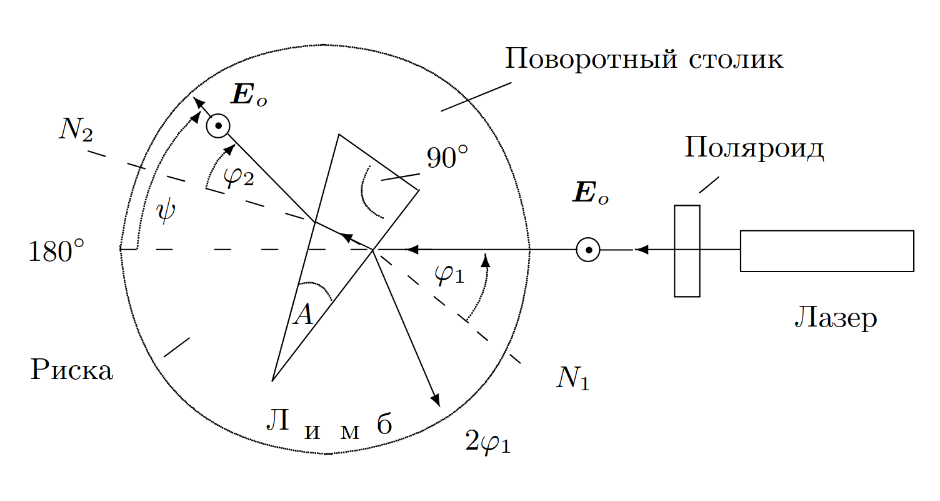
\includegraphics[width=0.8\textwidth]{1.png}
\caption{Экспериментальная установка}
\label{}
\end{figure}

Затем определим зависимость преломленного угла от катета и гипотинузы от наклона призмы:

\begin{figure}[!h]
\centering
\caption{Сравнение отражений от катета и гипотенузы}

\begin{minipage}[!h]{0.45\textwidth}
\centering
\begin{tabular}{|c|c|}
\hline
$\alpha$ & $2 \phi_1$ \\
\hline
10°  &  64.5° \\
20°  &  69.4° \\
30°  &  74.5° \\
40°  &  79.2° \\
50°  &  84.4° \\
60°  &  89.4° \\
70°  &  94.5° \\
80°  &  99.5° \\
90°  & 104.0° \\
100° & 109.0° \\
110° & 114.2° \\
120° & 120.0° \\
130° & 124.0° \\
140° & 129.0° \\
\hline
\end{tabular}

\vspace{0.5em}
Отражение от катета
\end{minipage}
\hfill
\begin{minipage}{0.45\textwidth}
\centering
\begin{tabular}{|c|c|}
\hline
$\alpha$ & $2 \phi_2$ \\
\hline
10°  & 282°   \\
20°  & 287.8° \\
30°  & 292.8° \\
40°  & 298°   \\
50°  & 303°   \\
60°  & 307.5° \\
70°  & 312°   \\
80°  & 318°   \\
90°  & 323°   \\
100° & 328°   \\
110° & 333°   \\
120° & 338°   \\
130° & 343°   \\
140° & 347.5° \\
\hline
\end{tabular}

\vspace{0.5em}
Отражение от гипотенузы
\end{minipage}

\end{figure}

Также определим угол $A$ как разница положений рисок в положениях, когда луч отраженный от катета и гипотинузы попадают обратно в 0:

\begin{equation}
    A = 180 - \phi_1 - \phi_2 = (38.0 \pm 0.5)\text{°}
\end{equation}

\noindent Показатель преломления призмы может быть найден как
\begin{equation}
    n = \frac{1}{\sin A} \sqrt{\sin^2\varphi_1 + \sin^2\varphi_2 + 2\sin\varphi_1\sin\varphi_2\cos A}.
\end{equation}

\noindent Для призмы из изотропного матреиала в случае, когда $\varphi_1 = \varphi_2$, показатель преломления может быть рассчитан по формуле
\begin{equation}
    n = \frac{ \sin\big( \frac{\psi_m + A}{2} \big) }{ \sin\big(\frac{A}{2}\big) },
\end{equation}
где $\psi_m$ -- угол наименьшего отклонения.

Далее снимем зависимость углов отклонения на выходе из призмы для обыкновенной и необыкновенной волны от угла падения луча на призму. Результаты этих измерений представлены в таблице 3.

\begin{table}[h!]
\centering
\begin{tabular}{|c|c|c|}
\hline
$2 \phi$ & $(180 + \psi_0)$ & $(180 + \psi_e)$ \\ \hline
10°  & 216.0° & 203.5° \\ \hline
20°  & 211.5° & 201.8° \\ \hline
30°  & 209.2° & 200.8° \\ \hline
40°  & 208.0° & 200.5° \\ \hline
50°  & 207.1° & 200.3° \\ \hline
60°  & 207.0° & 200.3° \\ \hline
70°  & 207.0° & 201.2° \\ \hline
80°  & 207.5° & 202.0° \\ \hline
90°  & 208.0° & 203.0° \\ \hline
100° & 209.5° & 204.0° \\ \hline
110° & 211.0° & 206.0° \\ \hline
120° & 213.0° & 208.2° \\ \hline
130° & 215.5° & 210.5° \\ \hline
140° & 218.5° & 213.5° \\ \hline
\end{tabular}
\caption{Зависимость углов отклонения от угла падения}
\end{table}

\noindent Из таблицы 3 также видим, что минимальные значение $\psi_o = 27.0^\circ$, минимальное значение $\psi_e = 20.3^\circ$. По этим величинам проведем вычисления показателся преломления, используя формулу:

\begin{equation}
    n = \frac{ \sin\big( \frac{\psi_m + A}{2} \big) }{ \sin\big(\frac{A}{2}\big) }
\end{equation}

\begin{equation}
    n_e = 1.65 \pm 0.05
\end{equation}

\begin{equation}
    n_o = 1.50 \pm 0.05
\end{equation}

Теперь построим график зависимости показателя преломления от $\cos(\theta)^2$:

\begin{figure}[!h]
\centering
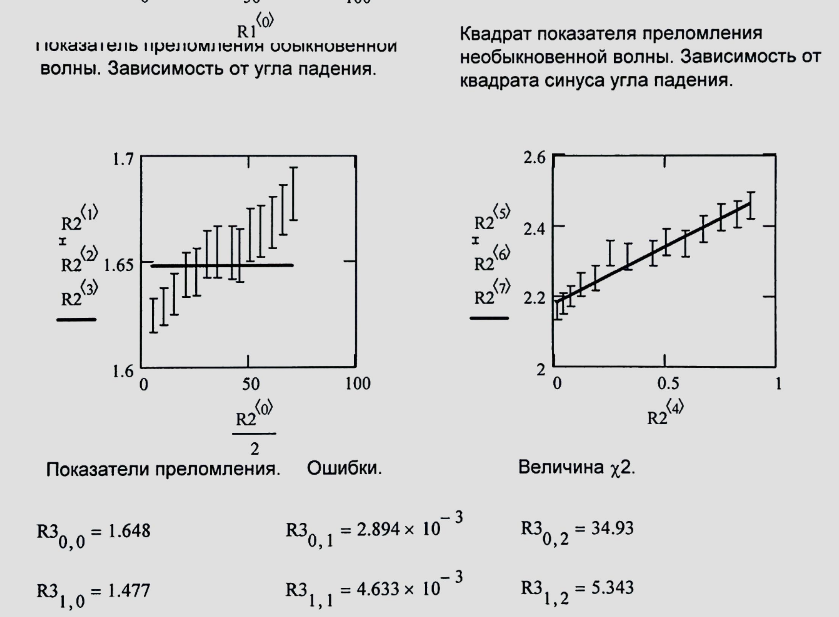
\includegraphics[width=0.8\textwidth]{2.png}
\caption{Результаты}
\label{}
\end{figure}

\section{Вывод}

В работе были изучена зависимость показателся преломления необыкновенной волны от направления ее распространения в двоякопреломляющем кристалле. Несколькими способами были определены значения главных показателей преломления обыкновенной и необыкновенной волны. 

\end{document}
